
\section[Methodology]{Methodology: Policy Learning Framework for Replay Scheduling}\label{paperD:sec:methodology}

In this section, we present an RL-based framework for learning replay scheduling policies that generalize across different CL scenarios. Our intuition is that there may exist general patterns regarding the replay scheduling, e.g., tasks that are harder or have been forgotten should be replayed more often. Moreover, the policy may non-trivially take task properties into consideration. Therefore, we aim to learn policies that select which tasks to replay from states representing the current task performance in the CL environments. The policy can then be applied for mitigating catastrophic forgetting in new CL scenarios. 


The CL environments are modeled using MDPs represented as tuples $E_i = (\gS_i, \gA, P_i, R_i, \mu_i, \gamma)$ sampled from a distribution of environments, such that $E_i \sim p(E)$ for $i=1, ..., K$. 
%We model the CL environments with MDPs represented by tuples $E_i = (\gS_i, \gA, P_i, R_i, \mu_i, \gamma)$ sampled from a distribution of CL environments, such that $E_i \sim p(E)$ for $i=1, ..., K$. 
We let the policy interact with a fixed set of environments $\gE^{(train)} = \{E_1, \dots, E_K\}$ sampled from the distribution $p(E)$ for training. 
Each environment $E_i$ contains of network $f_{\vphi}$ and $T$ datasets $\gD_{1:T}$ where the $t$-th dataset is learned at time step $t$. To generate diverse CL environments, we get environments with different network initializations of $f_{\vphi}$ and shuffled task orders in the dataset when we sample environments from $p(E)$. 
We define the state $s_t$ of the environment as the validation accuracies $A_{t, 1:t}^{val}$ on each seen task $1, ..., t$ from $f_{\vphi}$ at task $t$, i.e., $s_t = [A_{t, 1}, ..., A_{t, t}, 0, ..., 0]$, where we use zero-padding on future tasks. The action space $\gA$ is constructed as described in Appendix \ref{paperD:app:action_space}, such that the $a_t \in \gA$ corresponds to a task proportion $\vp_t$ used for sampling the replay memory $\gM_t$. We use a dense reward based on the average validation accuracies at task $t$, i.e., $r_{t} = \frac{1}{t}\sum_{i=1}^{t} A_{t, i}^{val}$. The state transition distribution $P_i(s' | s, a)$ represents the dynamics of the environment, which depend on the initialization of $f_{\vphi}$ and also the task order in the dataset. 

\begin{figure}[t]
	\centering
	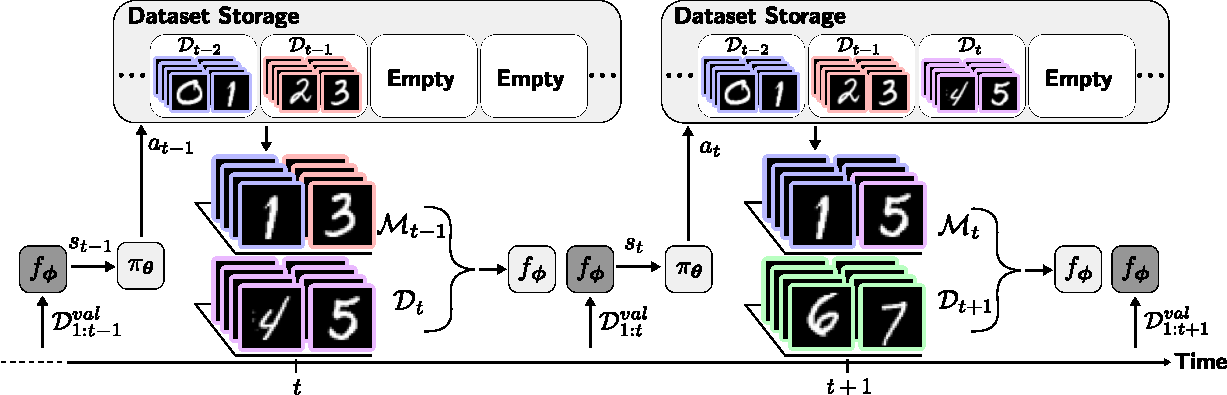
\includegraphics[width=0.95\textwidth]{Chapter1/figures/testing_size2.pdf}
	\caption{Illustration of the procedure of the proposed RL-based framework in a CL environment with Split MNIST. The goal is to mitigate catastrophic forgetting in the classifier $f_{\vphi}$ by composing replay memories $\gM$ with the replay scheduling policy $\pi_{\vtheta}$. The policy selects action $a$ determining which tasks to replay given the state $s$ represented as the validation task performances of $f_{\vphi}$. The colored border on the MNIST images indicates which task the data comes from. The classifier $f_{\vphi}$ is in evaluation mode when darker-shaded color over the box is used. %Pipeline of our proposed RL-based framework. 
	}
	\label{fig:rl_framework_pipeline}
	\vspace{-2mm}
\end{figure}

The procedure for training the policy goes as follows: 
The state $s_{t}$ is obtained by evaluating the network $f_{\vphi}$ on the validation sets $\gD_{1:t}^{val}$ after learning the $t$-th task from $\gD_t^{(train)}$. Action $a_{t}$ is selected under the policy $\pi_{\vtheta}(a | s_{t})$ parameterized by $\vtheta$. The action is converted into task proportion $\vp_t$ for sampling the replay memory $\gM_{t}$ from the historical datasets $\gD_{1:t}^{train}$. 
We then train classifier $f_{\vphi}$ with $\gD_{t+1}^{(train)}$ and $\gM_{t}$, and obtain the reward $r_{t+1}$ and the next state $s_{t+1}$ by evaluating $f_{\vphi}$ on the validation sets $\gD_{1:t}^{val}$. The collected transitions $(s_t, a_t, r_{t+1}, s_{t+1})$ are used for updating the policy. This procedure is followed until the final task $T$ after which we start a new episode. %for collecting experience.   
Figure \ref{fig:rl_framework_pipeline} shows an illustration of this procedure for using the learned replay scheduling policy in a CL environment with the Split MNIST dataset~\citeD{D:zenke2017continual}. The seen datasets are placed in the dataset storage to use for sampling replay memories given the actions from the policy $\pi_{\vtheta}$ for mitigating catastrophic forgetting at each time step.

We evaluate the learned policy by applying it to mitigate catastrophic forgetting in new CL environments at test time. To foster generalization across environments, we train the policy on multiple environments with different dynamics, e.g., task orders and datasets, to learn from diverse sets of training data. The goal for the agent is to maximize the sum of rewards in each training environment. %We evaluate the policy by using it for selecting which tasks to replay in new CL environments. 
At test time, the policy is applied on new CL classifiers and datasets in the test environments without added computational cost nor experience collection. In Section \ref{paperD:sec:experiments}, we test the policies generalization capability to new CL environments where the task orders and datasets are unseen during training.

